\documentclass[12pt,letterpaper,fleqn]{article}
\usepackage{fullpage}
\usepackage[top=2cm, bottom=4.5cm, left=2.5cm, right=2.5cm]{geometry}
\usepackage{amsmath,amsthm,amsfonts,amssymb,amscd}
\usepackage[utf8]{inputenc}
\usepackage{lastpage}
\usepackage{enumerate}
\usepackage{fancyhdr}
\usepackage{mathrsfs}
\usepackage{xcolor}
\usepackage{graphicx}
\usepackage{listings}
\usepackage{hyperref}
\usepackage{amsmath}
\usepackage{nccmath}
\usepackage{physics}
\usepackage{float}

\newcommand{\R}{\mathbb{R}}
\newcommand{\Q}{\mathbb{Q}}

\newcommand{\cent}{$^{\circ}$}
\newcommand{\delfrac}[2][y]{\frac{\partial #1}{\partial #2}}


\hypersetup{%
 colorlinks=true,
  linkcolor=blue,
  linkbordercolor={0 0 1}
}
 
\renewcommand\lstlistingname{Algorithm}
\renewcommand\lstlistlistingname{Algorithms}
\def\lstlistingautorefname{Alg.}

\lstdefinestyle{Python}{
    language        = Python,
    frame           = lines, 
    basicstyle      = \footnotesize,
    keywordstyle    = \color{blue},
    stringstyle     = \color{green},
    commentstyle    = \color{red}\ttfamily
}

\setlength{\parindent}{0.3in}
\setlength{\parskip}{0.05in}

% Edit these as appropriate
\newcommand\course{Física - Frente 1}
\newcommand\hwnumber{1}                  % <-- homework number
\newcommand\NetIDa{netid19823}           % <-- NetID of person #1
\newcommand\NetIDb{netid12038}           % <-- NetID of person #2 (Comment this line out for problem sets)

\pagestyle{fancyplain}
\headheight 35pt
%\lhead{\NetIDa}
%\lhead{\NetIDa\\\NetIDb}                 % <-- Comment this line out for problem sets (make sure you are person #1)
\chead{\textbf{\Large Pêndulo Simples (MHS) \hwnumber}}
\rhead{\course \\ Setembro/2020}
\lfoot{}
\cfoot{}
\rfoot{\small\thepage}
\headsep 1.5em

\begin{document}
\textit{Obs: Caso precise do valor da aceleração da gravidade em algum exercício: $g= 10\,m/s^2$ }
\begin{enumerate}
    \item Christiaan Huygens, em 1656, criou o relógio de pêndulo. Nesse dispositivo, a pontualidade baseia-se na regularidade das pequenas oscilações do pêndulo. Para manter a precisão desse relógio, diversos problemas foram contornados. Por exemplo, a haste passou por ajustes até que, no início do século XX, houve uma inovação, que foi sua fabricação usando uma liga metálica que se comporta regularmente em um largo intervalo de temperaturas.
    
    Desprezando a presença de forças dissipativas e considerando a aceleração da gravidade constante, para que esse tipo de relógio realize corretamente a contagem do tempo, é necessário que o(a):
    \begin{enumerate}
        \item Comprimento da haste seja mantido constante.
        \item Massa do corpo suspenso pela haste seja pequena.
        \item Material da haste possua alta condutividade térmica.
        \item Amplitude de oscilação seja constante a qualquer temperatura.
        \item Energia potencial gravitacional do corpo se mantenha constante.
    \end{enumerate}
    
    \item Dois sistemas oscilantes, um bloco pendurado em uma mola vertical e um pêndulo simples, são preparados na Terra de tal forma que possuam o mesmo período. Se os dois osciladores forem levados para a Estação Espacial Internacional (ISS), como se comportarão os seus períodos nesse ambiente de microgravidade?
    \begin{enumerate}
        \item Os períodos de ambos os osciladores se manterão os mesmo de quando estavam na Terra.
        \item O período do bloco pendurado na mola não sofrerá alteração, já o período do pêndulo deixará de ser o mesmo
        \item O período do pêndulo será o mesmo, no entanto o período do bloco pendurado na mola será alterado.
        \item Os períodos de ambos os osciladores sofrerão modificação em relação a quando estavam na Terra.
        \item n.d.a.
    \end{enumerate}
    
    
    \item Um relógio de pêndulo é construído tal que o seu pêndulo realize 3600 oscilações completas a cada hora. O relógio está descalibrado, de modo que o pêndulo oscila em um movimento harmônico simples de frequência angular igual a $5\pi/2$ rad/s. Nessa situação, ao final de 3600 oscilações completas do pêndulo terão se passado:
    \begin{enumerate}
        \item 32 min
        \item 45 min
        \item 48 min
        \item 52 min
        \item 56 min
    \end{enumerate}
    
    \item Um determinado tipo de sensor usado para medir forças, chamado de sensor piezoelétrico, é colocado em contato com a superficie de uma parede, onde se fixa uma mola. Dessa forma. pode-se medir a força exercida pela mola sobre a parede. Nesse contexto, um bloco, apoiado sobre uma superfície horizontal, é preso a outra extremidade de uma mola de constante elástica igual a 100 N/m. conforme ilustração a seguir.
    \begin{figure}[H]
        \centering
        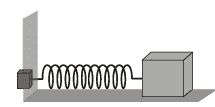
\includegraphics[width=0.5\textwidth]{enunciado_4.png}
    \end{figure}
    Nessa circunstância, fazendo-se com que esse bloco descreva um movimento harmônico simples, observa-se que a leitura do sensor é dada no gráfico a seguir
    \begin{figure}[H]
        \centering
        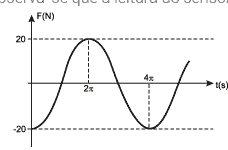
\includegraphics[width=0.5\textwidth]{ex_4.png}
    \end{figure}
    Com base nessas informações é correto afirmar que a velocidade máxima atingida pelo bloco, em m/s, é de:
    \begin{enumerate}
        \item 0,1
        \item 0,2
        \item 0,4
        \item 0,8
        \item 1,0
    \end{enumerate}
    \textit{Dica e encaminhamento: Lembrar que no ponto de aceleração máxima da massa, a velocidade dela é 0. Com isso, calcular a deformação da mola e, após isso, calcular a energia potencial da mola. Por último, aplicar o princípio de conservação de energia para achar a velocidade por meio da energia cinética.}
    
    \item Construíram-se três pêndulos simples utilizando-se bolinhas e fios finos.

\begin{itemize}
    \item Pêndulo 1 – Uma bolinha de  50g presa à extremidade de um fio com 40 cm de comprimento.
\item Pêndulo 2 – Uma bolinha de 100g presa à extremidade de um fio com 80 cm de comprimento.
\item Pêndulo 3 – Uma bolinha de 25 g presa à extremidade de um fio com 40 cm de comprimento.
\end{itemize}

Os três pêndulos foram postos a oscilar separadamente durante 10 segundos e foi anotado o número de oscilações completas que cada um deles realizou nesse intervalo de tempo. É CORRETO afirmar:
\begin{enumerate}
    \item O pêndulo 3 oscilou mais vezes que o pêndulo 1.
    \item O pêndulo 2 oscilou mais vezes que os outros dois.
    \item Os pêndulos 1 e 3 oscilaram  o mesmo número de vezes.
    \item O pêndulo 1 oscilou um maior número de vezes que os outros dois.
\end{enumerate}

\item Oscilações são movimentos que se repetem. Geralmente estes são amortecidos, ou seja, reduzem-se gradualmente, transformando energia mecânica em energia térmica, sendo que no mundo real não é possível eliminar as perdas, mas é possível recarregar a energia. No movimento harmônico, essas oscilações se repetem periodicamente com a mesma freqüência.

Se um menino estiver se balançando em uma corda pendurada em uma árvore, recarregando a energia perdida com o movimento das pernas e fazendo 40 oscilações em um minuto, é CORRETO afirmar que (considere $g = 10 m/s^2$ e $\pi$ = 3,14)
\begin{enumerate}
    \item   seu período será de 60 segundos.
    \item o período é numericamente igual à freqüência.
    \item o comprimento da corda é de 3 m.
    \item o período será o triplo, se o comprimento da corda for triplicado.
    \item a freqüência é de 2/3 Hertz.
\end{enumerate}
\item Um balde contendo água é amarrado na extremidade de uma corda cuja outra extremidade está presa ao teto. O balde é posto para oscilar e o sistema pode ser considerado como um pêndulo simples. No entanto, há um pequeno furo no fundo do balde e, enquanto o balde oscila, a quantidade de água neste vai diminuindo. Despreze qualquer força de atrito. Sendo 'T' o período e 'E' a energia mecânica do pêndulo, enquanto este oscila, é CORRETO afirmar que:

\begin{enumerate}
    \item T e E não variam.
    \item T não varia e E diminui.
    \item T e E diminuem.
    \item T diminui e E não varia.
\end{enumerate}

\item O pêndulo simples é um sistema idealizado, consistindo em uma partícula suspensa por um cabo leve inextensível que, quando puxado para um dos lados de sua posição de equilíbrio e liberado, oscila no plano vertical sob a influência da força gravitacional. Considere um pêndulo simples com comprimento de 9,0m e que executa 20 oscilações completas em 2,0 min, em um determinado local.

Com base nessas informações, constata-se que o módulo da aceleração da gravidade nesse local, em metros por segundo ao quadrado, é, aproximadamente, igual a:

\textit{Note e adote: $\pi =3,14$}
\begin{enumerate}
    \item 9,53
    \item 9,61
    \item 9,87
    \item 9,98
    \item 10,05
\end{enumerate}

\item Considerando um corpo em movimento harmônico simples - MHS, descrevendo uma trajetória retilínea onde X representa o centro do movimento, analise as alternativas a seguir e assinale a INCORRETA.

\begin{enumerate}
    \item O movimento progressivo é acelerado em parte e retardado em parte.
    \item O movimento retrógrado é acelerado em parte e retardado em parte.
    \item Em um ponto escolhido arbitrariamente, o móvel passa com velocidades sempre iguais em valor absoluto.
    \item A força que age no corpo é sempre contrária à velocidade.
    \item A força que age no corpo é sempre contrária à elongação.
\end{enumerate}
\end{enumerate}
\newpage
\section*{GABARITO}

\begin{enumerate}
    \item (a) - Pela fórmuala do período do pêndulo, o único fator do pêndulo que entra é o comprimento da haste.
    \item (b) - O período da oscilação massa-mola não muda, porque ela só depende da constante da mola (k) e da massa (m). Já o período do pêndulo muda, pois a força gravitacional mudou, logo a aceleração da gravidade (g) é outra, e a aceleração da gravidade entra na conta do período do pêndulo
    \item (c) - Pela fórmula da frequência angular:
    \begin{align*}
        \omega = \frac{2\pi}{T} \implies \frac{5\pi}{2} = \frac{2\pi}{T} \implies T = \frac{4}{5}\,s
    \end{align*}
    Logo, o tempo total será o tempo de uma oscilação vezes o número de oscilações:
    \begin{equation*}
        \Delta\,t = \frac{4}{5}.3600 = 2880\,s = 48\,min
    \end{equation*}
    \item (a) - Seguindo a indicação do exercício: O ponto de aceleração máxima é o mesmo ponto em que a força é máxima, logo, quando a força é de 20 N. Como é uma mola, pela Lei de Hooke, temos que:
    \begin{align*}
        \abs{F} = k\,x \implies 20 = 100\,x \implies x = 0,2\,m
    \end{align*}
    Calculando a energia potencial da mola quando a deformação da mola é máxima:
    \begin{align*}
        U_1 = \frac{k\,x^2}{2} \implies \frac{100\,0,2^2}{2} = 2\,J
    \end{align*}
    Aplicando o princípio de conservação de energia entre os instantes em que a deformação da mola é máxima e o instante em que a mola está relaxada:
    \begin{equation*}
        U_{1} + T_1 = U_2 + T_2
    \end{equation*}
    Como na deformação máxima, a massa está parada, então $T_1=0$. Quando a mola está relaxada, a deformação dela é 0, então $U_2 = 0$. Logo:
    \begin{equation*}
        2 = T_2 \implies 2 = \frac{m\,v^2}{2}
    \end{equation*}
    A quantidade que falta é achar a massa, mas isso é possível encontrar via o gráfico e a fórmula do período do sistema massa-mola. Pelo gráfico, percebemos que o sistema volta a repetir após $4\pi$ s, então
    \begin{equation*}
        T = 2\pi\sqrt{\frac{m}{k}} \implies 4\pi = 2\pi\sqrt{\frac{m}{100}} \implies 2 = \frac{\sqrt{m}}{10} \implies m = 20^2 = 400\,kg
    \end{equation*}
    
    De volta na fórmula da energia cinética:
    \begin{align*}
        2 = \frac{mv^2}{2} \implies v^2 = \frac{4}{400} = \frac{1}{100} \implies v= \sqrt{\frac{1}{100}} = \frac{1}{10} \implies \boxed{v = 0,1\,m/s}
    \end{align*}
    \item (c) - O período do pêndulo só depende do tamanho do fio, então os pêndulos 1 e 3 possuem o mesmo período de tempo, logo eles oscilaram o mesmo número de vezes. O pêndulo 2 possui um período de tempo maior, pois o fio é maior. Dessa forma, o pêndulo oscila menos durante 10 s.
    \item (e) - Lembrar que 1 min = 60 s, então, o período de cada oscilação é:
    \begin{equation*}
        \delta\,t = N\,T = 60 = 40\,T \implies T=\frac{60}{40} =\frac{3}{2}\,s
    \end{equation*}
    Porém, a frequência de oscilação é o inverso do período do movimento:
    \begin{equation*}
        f = \frac{1}{T} = f = \frac{1}{\frac{3}{2}} \implies = \frac{2}{3}\,Hz
    \end{equation*}
    \item (b) - O período de oscilação só depende do comprimento do pêndulo, independe da massa de água no balde. Mas a energia mecânica (soma das energias potenciais gravitacional ($U = mgh$) e energia cinética $\left(T=\frac{mv^2}{2}\right)$) dependem da massa e, por isso, a energia mecânica diminui ao longo do tempo.
    \item (c) - Como o pêndulo faz 20 oscilações em 2 minutos (120 s), então:
    \begin{equation*}
        120 = 20\,T \implies T = 6\,s    
    \end{equation*}
    Usando isso na fórmula do período de um pêndulo:
    \begin{equation*}
        T = 2\pi\sqrt{\frac{L}{g}} \implies 6 = 2\pi\sqrt{\frac{9}{g}} \implies \frac{3}{\pi} = \sqrt{\frac{9}{g}} \implies \frac{9}{g} = \frac{9}{\pi^2} \implies g = \pi^2
    \end{equation*}
    Tomando $\pi\approx 3,14$ e fazendo as contas:
    \begin{equation*}
        g \approx 9,87\,m/s^2
    \end{equation*}
    \item (d) - há 2 ponto em que a força está no mesmo sentido do que a velocidade: é quando o objeto acabou de sair de um dos extremos do movimento.
\end{enumerate}
\end{document}
